\subsection{Basics}
\begin{frame}
        \frametitle{Acquiring Moltres}
             \texttt{git clone https://github.com/arfc/moltres}\\
        \texttt{cd moltres}\\
        \texttt{git submodule init}\\
        \texttt{git submodule update}\\
\end{frame}



\begin{frame}
  \frametitle{Moltres (coupling in MOOSE)}
   \begin{block}{Moltres principal concept \cite{lindsay_introduction_2018}}
     \begin{itemize}
        \item Moltres is built on top of the Multi-physics Object-Oriented
Simulation Environment (MOOSE)
		\item MOOSE interfaces with libMesh to discretize simulation volume
into finite elements
		\item Provides interface for coding residuals that correspond to weak
form of governing PDEs; also interface for coding Jacobians $\Rightarrow$
more accurate Jacobians $\Rightarrow$ more efficient convergence
		\item Residuals and Jacobians send to PetSc which handles solution of resulting non-linear system of algebraic equations
     \end{itemize}
    \end{block}
               \begin{figure}[t]
                \vspace*{-0.15in}
                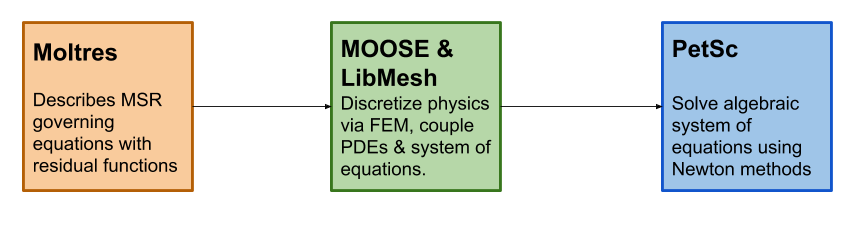
\includegraphics[height=0.24\textwidth]{./images/moltres-moose-diag.png}
                \vspace*{-0.1in}
                \caption{Moltres principal scheme}
               \end{figure}   
\end{frame}

\begin{frame}
	\frametitle{Intro to Moltres}
    	\begin{itemize}
			\item Liquid-fueled, molten salt reactors
			\item Multi-group diffusion (arbitrary number of groups)
			\item Advective movement of delayed neutron precursors
			\item Reynolds-averaged Navier-Stokes thermal hydraulics
			\item 2D axisymmetric
			\item 3D unstructured or structured
	    \end{itemize}
\end{frame}

\subsection{Kernels}
\begin{frame}
        \frametitle{Moltres Kernels}
        \footnotesize{Typical symbols (e.g. $\phi=\mbox{ neutron flux}$, 
                $T=\mbox{ temperature}$, and $C=\mbox{ precursor 
                concentrations}$).

\begin{align*}
\intertext{CoupledFissionEigenKernel} 
&\frac{\chi_g^p}{k} \sum_{g' = 1}^G (1 -
        \beta) \nu \Sigma_{g'}^f \phi_{g'}\\
\intertext{CoupledFissionKernel} 
&\chi_g^p \sum_{g' = 1}^G (1 -
        \beta) \nu \Sigma_{g'}^f \phi_{g'}\\
\intertext{CoupledScalarAdvection} 
&\nabla \cdot \vec{a} u\\
\intertext{DelayedNeutronSource} 
&\chi_g^d \sum_i^I \lambda_i C_i\\
\intertext{DivFreeCoupledScalarAdvection}
&\vec{a} \cdot \nabla u
\end{align*}}
\end{frame}

\begin{frame}
        \frametitle{Moltres Kernels}
        \footnotesize{
\begin{align*}
\intertext{FissionHeatSource}
&\frac{P}{\int_{\partial V} \sum_{g' = 1}^G \nu \Sigma_{g'}^f \phi_{g'} dV}
\sum_{g' = 1}^G \nu \Sigma_{g'}^f \phi_{g'}\\
\intertext{GammaHeatSource} &\gamma Q_f\\
\end{align*}

where $\gamma$ is a factor
representing heat dissipation by gamma and neutron irradiation in the moderator
and $Q_f$ is given by:

\begin{align*}
\sum_{g=1}^G \epsilon_{f,g}\Sigma_{f,g}\phi_g\\
\end{align*}

with $\epsilon_{f,g}$ being the amount of heat per fission event.}
\end{frame}

\begin{frame}
        \frametitle{Moltres Kernels}
        \footnotesize{
\begin{align*}
\intertext{GroupDiffusion}
& \nabla \cdot D_g
        \nabla \phi_g\\
\intertext{InScatter}
&\sum_{g \ne g'}^G
        \Sigma_{g'\rightarrow g}^s \phi_{g'}\\
\intertext{NtTimeDerivative}
&\frac{1}{v_g}\frac{\partial \phi_g}{\partial t}\\
\intertext{PrecursorDecay}
&\lambda_i C_i\\
\intertext{PrecursorSource}
&\sum_{g'= 1}^G \beta_i \nu
        \Sigma_{g'}^f \phi_{g'}\\
\end{align*}
}
\end{frame}

\begin{frame}
        \frametitle{Moltres Kernels}
        \footnotesize{
\begin{align*}
\intertext{ScalarAdvectionArtDiff}
&\nabla \cdot -\delta \nabla u\\
\end{align*}
where $\delta$ is an artificial diffusion coefficient, with $\vec{a}$ the 
        advection velocity and $h_{max}$ the maximum element length dimension:
\begin{align*}
&\delta = \frac{|\vec{a}| h_{max}}{2}\\
\end{align*}
\begin{align*}
\intertext{ScalarTransportTimeDerivative}
&\frac{\partial u}{\partial t}\\
\intertext{SelfFissionEigenKernel}
&\frac{-\nu_f \Sigma_f \phi}{k}\\
\intertext{SigmaR}
&\Sigma_g^r \phi_g\\
\intertext{TransientFissionHeatSource}
&\sum_{g=1}^G \epsilon_{f,g}\Sigma_{f,g}\phi_g\\
\end{align*}
        }
\end{frame}


%\begin{frame}
%  \frametitle{Moltres Kernels}
%    \begin{columns}
%    \column[t]{6cm}
%               \begin{figure}[t]
%                  \vspace*{-0.15in}
%                 \hspace*{-0.35in}
%                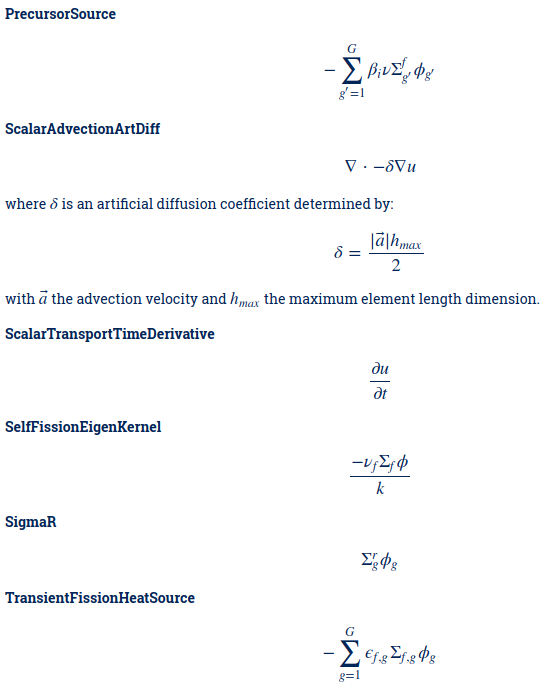
\includegraphics[height=1.15\textwidth]{./images/kernels4.png}
%               \end{figure}   
%
%    \column[t]{6cm}
%	\begin{itemize}
%		\item Kernels are individual pieces of governing equations
%		\item Modular (i.e. ``Diffusion" kernel could be used equally well to describe conduction or viscous shear)
%	\end{itemize}
%    \end{columns}  
%  
%\end{frame}
%
%\begin{frame}
%  \frametitle{Moltres Kernels (2)}
%               \begin{figure}[t]
%               \vspace*{-0.1in}
%                 \hspace*{-0.35in}
%                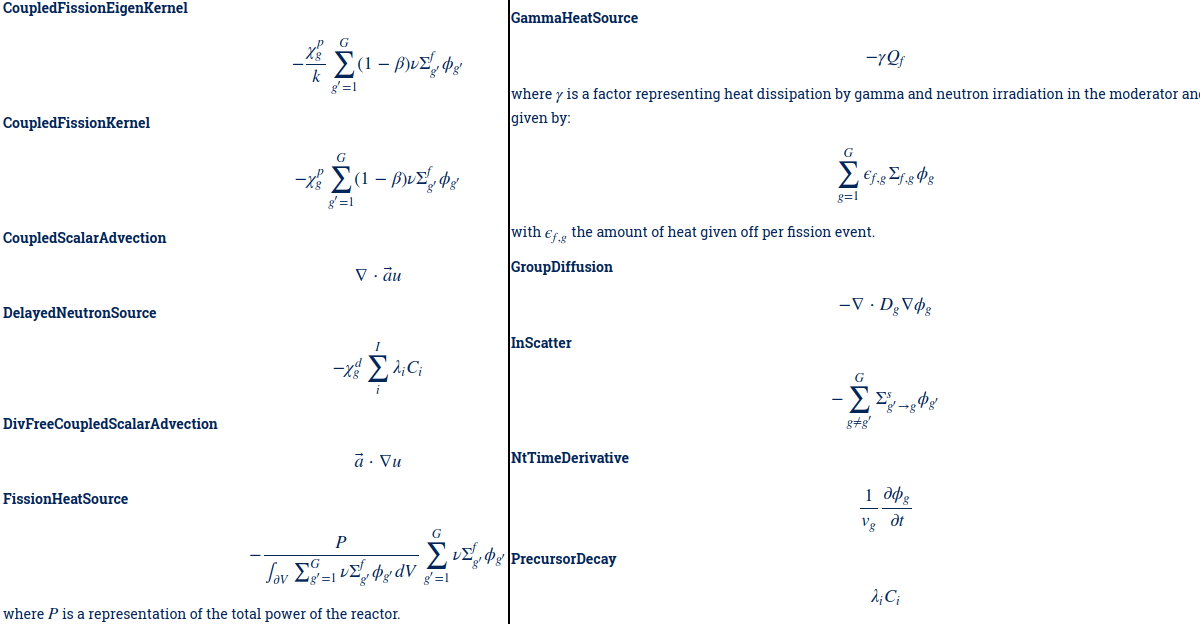
\includegraphics[height=0.6\textwidth]{./images/kernels11.png}
%               \end{figure}   
%\end{frame}

\subsection{Governing Equations}

\begin{frame}
  \frametitle{Governing Equations}
      \begin{block}{Time-dependent multi-group diffusion}
              \begin{figure}[t]
               \hspace*{-0.25in}
                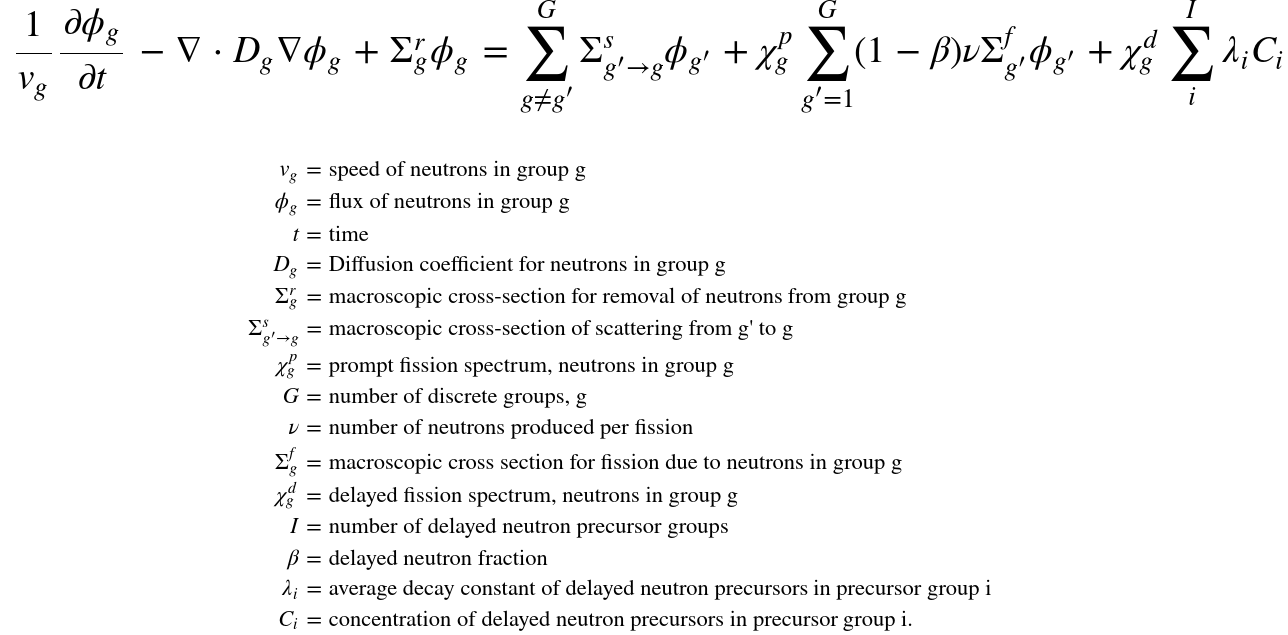
\includegraphics[height=0.55\textwidth]{./images/diffusion.png}
               \end{figure}   
      \end{block}
\end{frame}

\begin{frame}
  \frametitle{Governing Equations (2)}
     \begin{block}{Delayed neutron precursors}
               \begin{figure}[t]
                 \vspace*{-0.05in}
                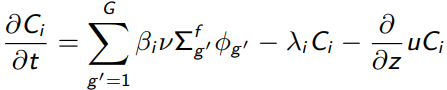
\includegraphics[height=0.07\textwidth]{./images/delayed_neutrons.png}
               \end{figure}   
     \end{block}
     
     \begin{block}{Heat conduction-convection with fission source in fuel}
              \begin{figure}[t]
                 \vspace*{-0.05in}
                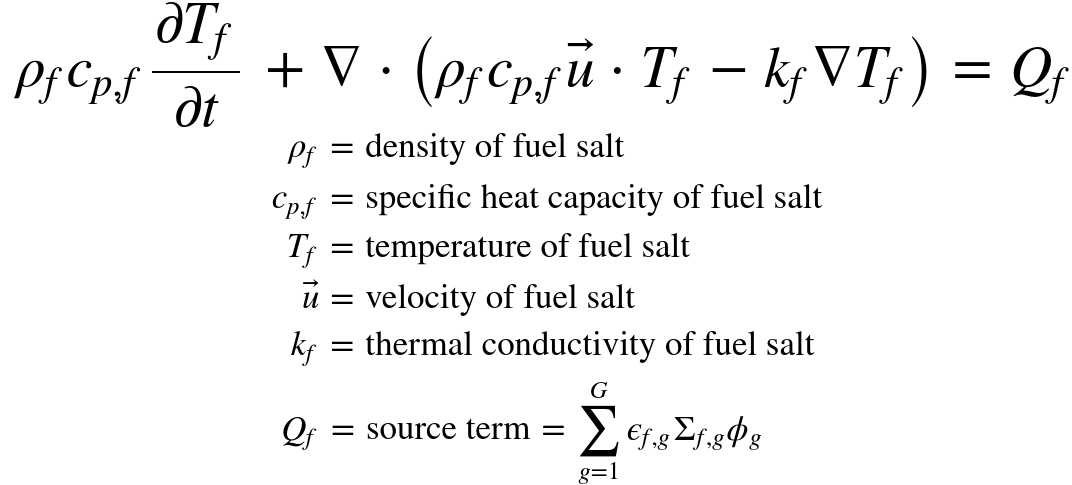
\includegraphics[height=0.21\textwidth]{./images/fuel_temp.png}
               \end{figure}        
	\end{block}
	
     \begin{block}{Heat conduction with option for irradiation source in moderator}
              \begin{figure}[t]
                 \vspace*{-0.05in}
                 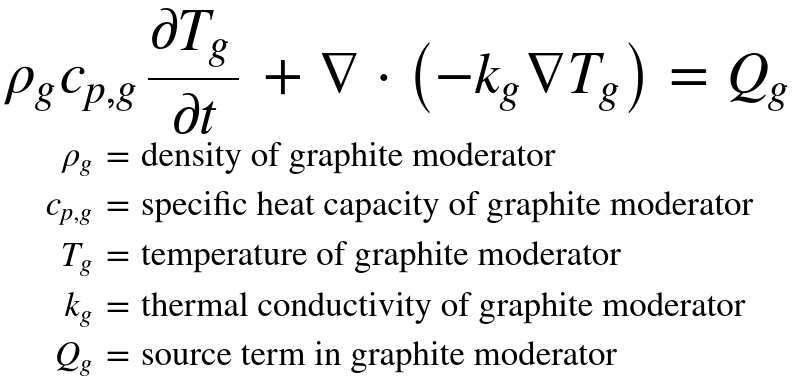
\includegraphics[height=0.17\textwidth]{./images/moder_temp.png}
               \end{figure}        
	\end{block}
\end{frame}

\begin{frame}
  \frametitle{Moltres \gls{MSRE} Simulations}
              \begin{figure}[t]
               \hspace*{-0.25in}
                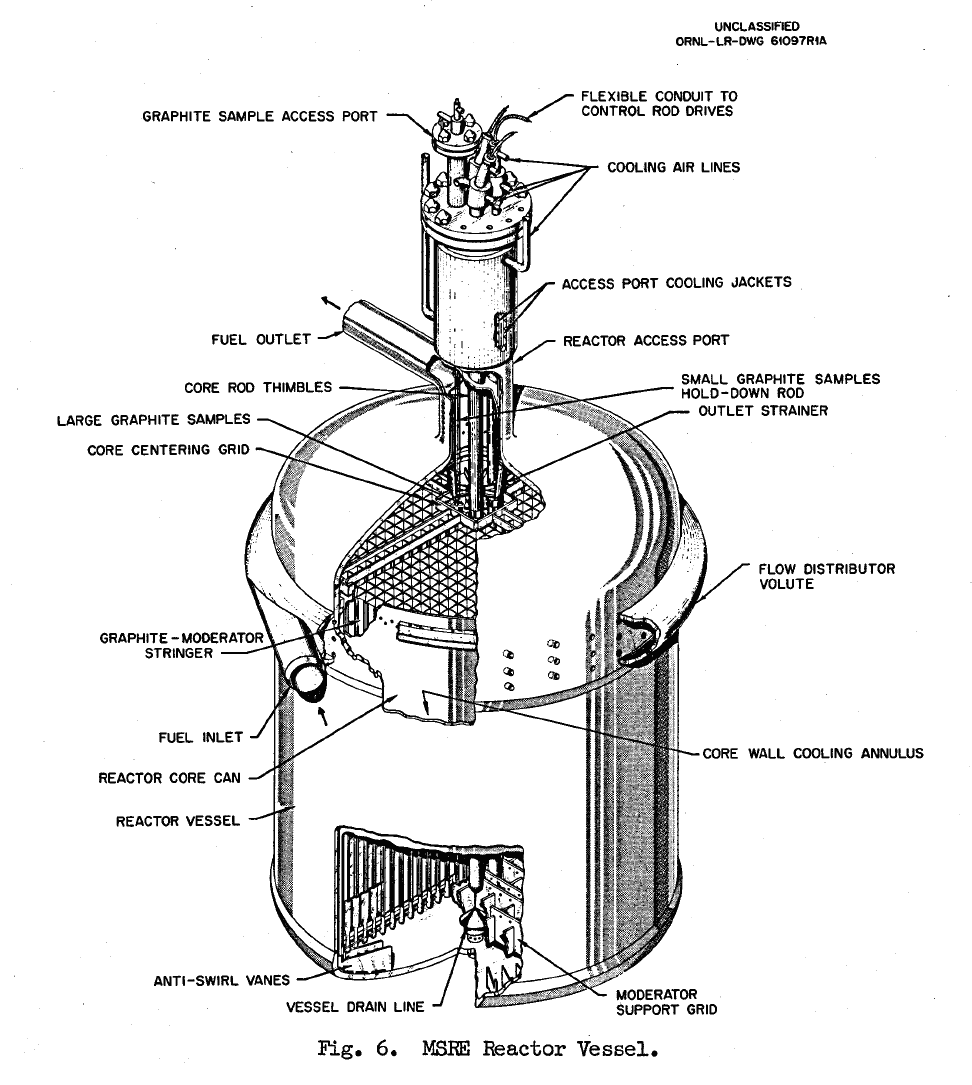
\includegraphics[height=0.65\textwidth]{./images/msre.png}
               \end{figure}   
\end{frame}

%\begin{frame}
%  \frametitle{Moltres MSRE Simulation: Input Data}
%     \begin{block}{Main input parameters \cite{lindsay_introduction_2018}}
%     	\begin{itemize}
%     		\item 22.5\% fuel volume fraction
%     		\item 2D axisymmetric and 3D core geometries derived 
%                        Group constants generated with SERPENT or NEWT (3D or 2D)
%     	\end{itemize}
%              \begin{figure}[t]
%                 \vspace*{-0.15in}
%                 \hspace*{-2.0in}
%                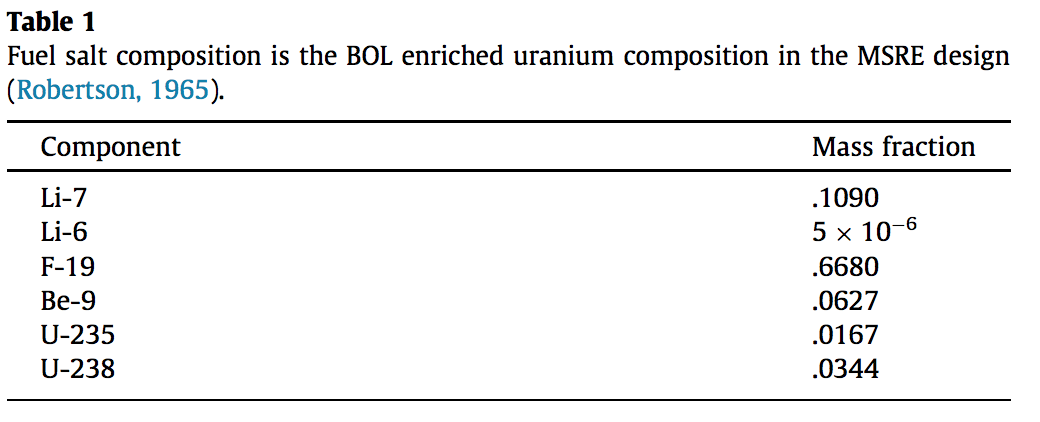
\includegraphics[height=0.2\textwidth]{./images/moltres-composition.png}
%               \end{figure}     
%               \begin{figure}[t]
%                 \vspace*{-0.25in}
%                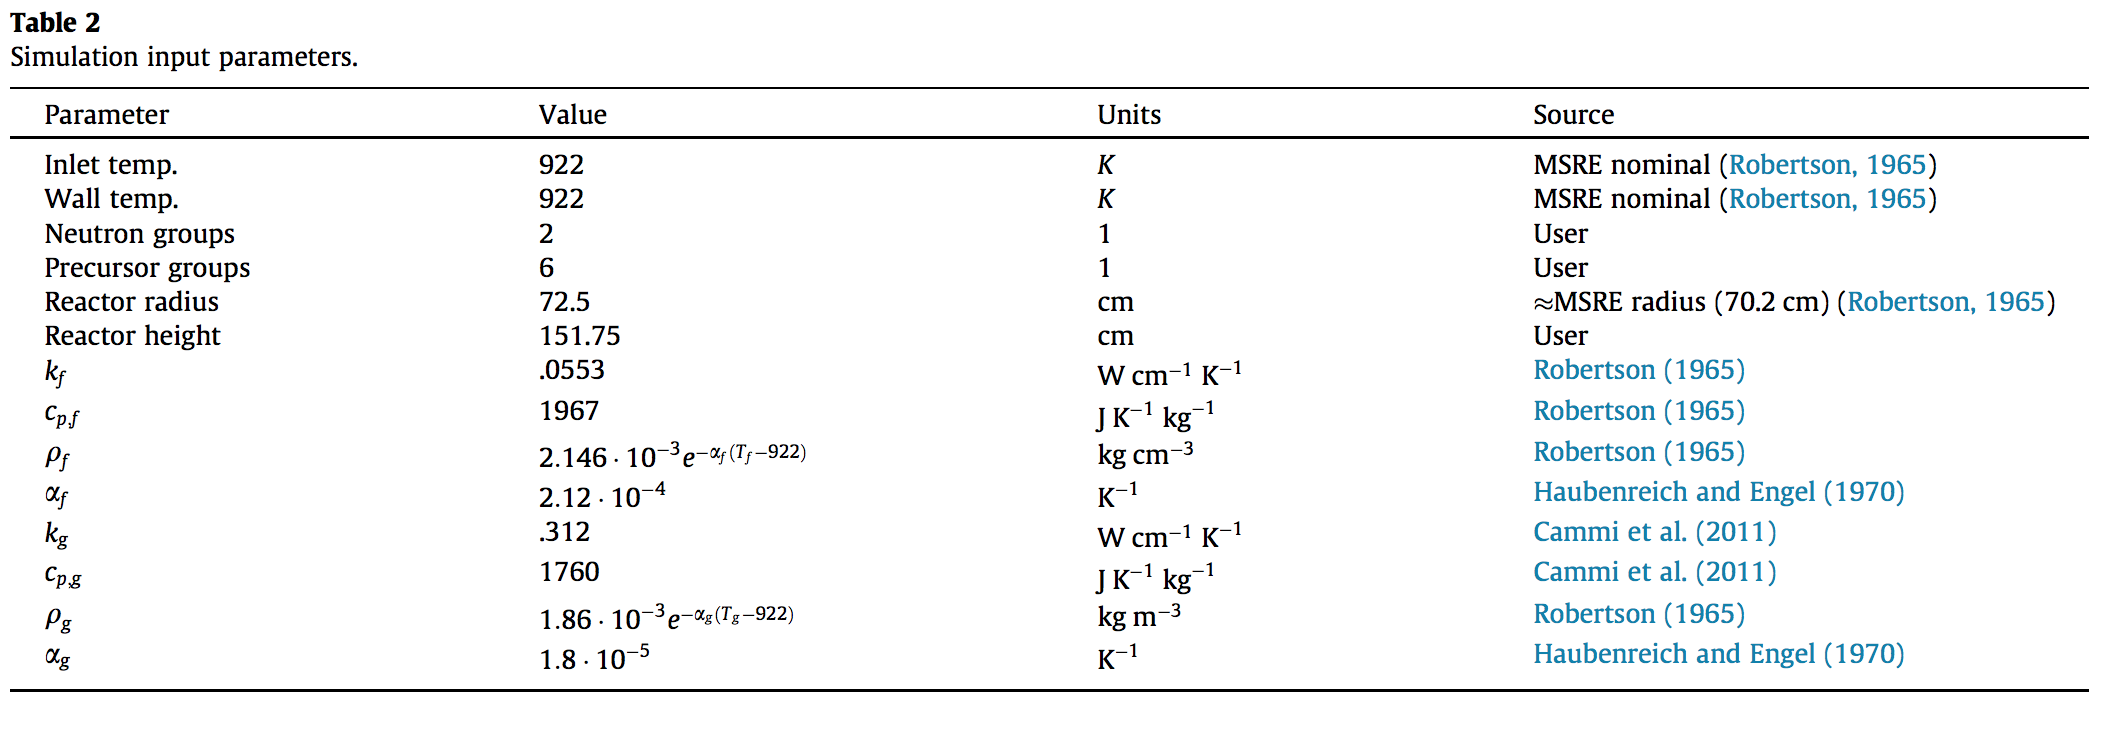
\includegraphics[height=0.33\textwidth]{./images/moltres-input.png}
%               \end{figure}   
%	\end{block}
%	
%\end{frame}
